\documentclass[10pt]{article}
%\documentclass[prd,twocolumn,showpcs,amsmath,amssymb,nofootinbib,preprintnumbers,balancelastpage,longbibliography]{revtex4-1}
\usepackage[a4paper, left=1.5cm, right=1.5cm, top=3.5cm]{geometry}
\usepackage[ngerman]{babel}
\usepackage[]{graphicx}
\usepackage{multicol}
\usepackage{amssymb}
\usepackage{inputenc}
\usepackage{breqn}
\usepackage{titlesec}
\usepackage{wrapfig}
\usepackage{blindtext}
\usepackage{lipsum}
\usepackage{caption}
\usepackage{listings}
\usepackage{fancyhdr}
\usepackage{nopageno}
\usepackage{bm}
\usepackage{authblk}
\usepackage{amsmath}
\usepackage{mathtools}
\usepackage{bm}
\usepackage[ISO]{diffcoeff}
\usepackage{xcolor}
\usepackage{csquotes}
\usepackage{siunitx}
\usepackage{circuitikz}
\usepackage{biblatex}
\usepackage{hyperref}

%%\pdfoutput=1
\usepackage{epsfig}
\usepackage{amsmath}
\usepackage{bm}
\usepackage{times}
%\usepackage{cite}
\usepackage{physics}
\usepackage{graphicx}
\usepackage{color}
\usepackage{slashed}
\usepackage{graphicx}
\usepackage{amsmath}
\usepackage{mathrsfs}
\usepackage{tikz}
\usetikzlibrary{positioning,shapes}
\usepackage{relsize,caption} 
\usepackage[latin1]{inputenc}
\usepackage{textcomp}
\usepackage[T1]{fontenc}
\usepackage{tikz}

%\usepackage{biblatex}
\usepackage{hyperref}

\usetikzlibrary{trees}
\usetikzlibrary{decorations.pathmorphing}
\usetikzlibrary{decorations.markings}
\usetikzlibrary{positioning,arrows}
\usetikzlibrary{decorations.pathmorphing}
\usetikzlibrary{decorations.markings}
\usetikzlibrary{decorations.pathreplacing,calc}
\usetikzlibrary{decorations.pathmorphing,decorations.markings,trees,positioning,arrows}   
\newif\ifmirrorsemicircle

\fancyhf[]{}

\addbibresource{latex.bib}

\newenvironment{Figure}
  {\par\medskip\noindent\minipage{\linewidth}}
  {\endminipage\par\medskip}

\begin{titlepage}
    \title{Praktikum 4 -- Versuch 443: Kernmagnetische Relaxation}
    \author[1]{Jonas Wortmann\thanks{s02jwort@uni-bonn.de}}
    \author[1]{Angelo V. Brade\thanks{s72abrad@uni-bonn.de}}
    \affil[1]{Rheinische Friedrich-Wilhelms-Universität Bonn}
    \date{\today}
\end{titlepage}

\begin{document}
\pagenumbering{gobble}
\maketitle
\newpage

\tableofcontents
\newpage

\pagenumbering{arabic}

\pagestyle{fancy}
\fancyhead[R]{\thepage}
\fancyhead[L]{\leftmark}


\begin{multicols}{2}
  \section{Einführung}
  Die Kernmagnetische Relaxation ist die Grundlage vieler moderner Messtechniken der Medizin, Chemie und Physik. Sie wird gebrauch, um z.B. MRTs oder NMRs durchzuführen. In diesem Versuch bestimmen wir die Rabioszillation und die longitudinale bzw. transversale Relaxationszeit $T_1$ und $T_2$. Diese sind materialspezifische Größen, die z.B. dessen Identifikation ermöglichen. Wir legen hier allerdings den Schwerpunkt auf die Messung der Größen selbst.
  \section{Aufbau}
  Bei dem Aufbau handelt es sich um eine Verkabelung der vier verschiedenen Geräte: MAGNET, PS2 Controller, Mainframe und das digitale Oszilloskop.
  
  Der \textbf{Magnet} ist eine Permanentmagnet, der ein homogenes Magnetfeld erzeugt. Dieser kann mit einer Helmholzspule, also zwei Spulen die genau um ihren Radius voneinander entfernt sind, ein homogenes Magnetfeld erzeugen, wenn die Spulen symmetrisch, also '$-+$' und '$-+$', oder ein Gradientenfeld, wenn die Spulen antisymmterisch, also '$-+$' und '$+-$', gepolt sind, erzeugen. Zusätzlich beinhaltet er eine sog.\ Sample Coil, die ein Magnetfeld innerhalb der Appartur messen kann. Solch ein Magnetfeld würde in unserem Fall eine Probe erzeugen, welche in die Mitte eingeführt werden kann, sodass sie umgeben von der Sample Coil und der Helmholzspulen ist. Das Innere ist nochmal in Abb. \ref{fig:mag} gezeigt.
\begin{Figure}
  \centering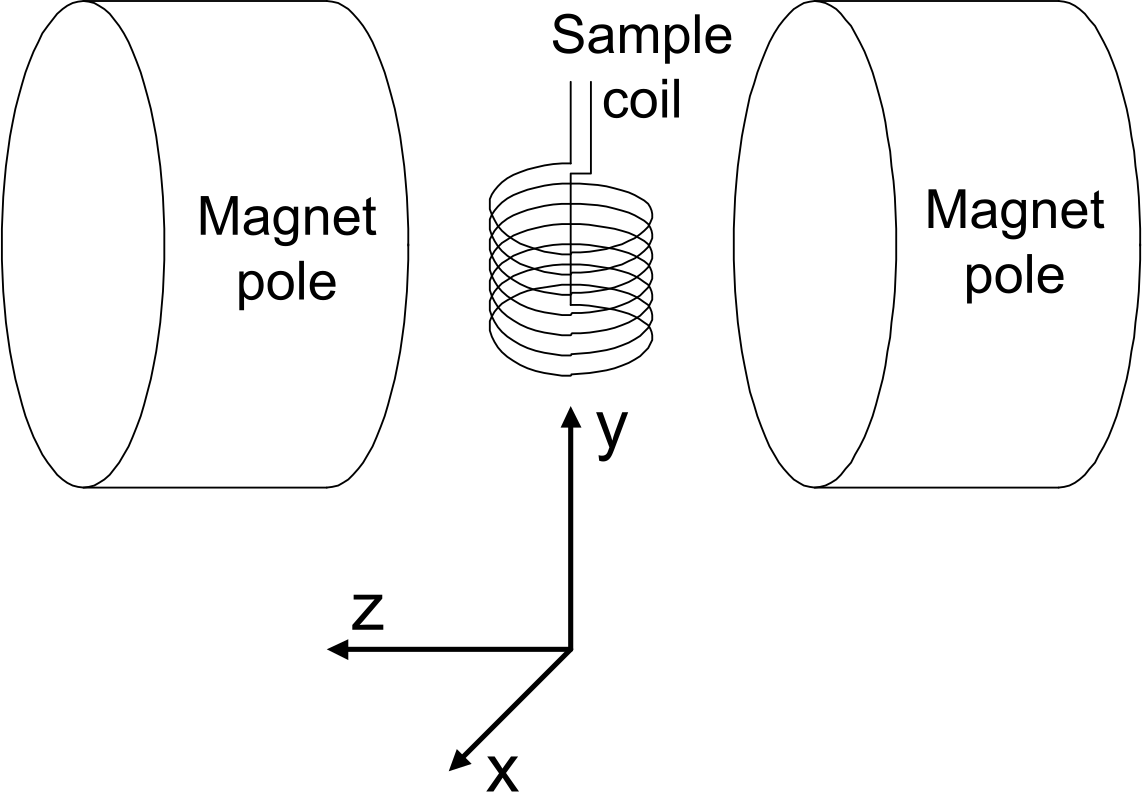
\includegraphics[width=0.8\textwidth]{magnet_aufbau.png}
  \captionof{figure}{Aufbau vom Magneten.\cite{TeachSpin}}
  \label{fig:mag}
\end{Figure}

  Der \textbf{PS2 Controller} reguliert den Magneten auf die Raumtemperatur, um Imperfektionen/Inhomogenitäten zu reduzieren. Außerdem lässt er über die Stromzufuhr der Helmholzspulen dessen Gradienten einstellen. Dafür sind uns die Regler für $X$, $Y$, $Z$ und $Z^2$ gegeben. Diese sind später bei der Justage für $\frac{\pi}{2}$- bzw. $\pi$-Pulse iterativ zu optimieren. Zusätzslich lässt sich neben der Sträke auch das Vorzeichen der Gradienten mithilfe eines jeweiligen Schalters einstellen.

  Der \textbf{Mainframe} enthält einen Receiver, der ein einkommendes Signal zur Darstellung am Oszilloskop verstärken kann, einen Synthesizer, der die Frequenz des zirkular polarisierten Mangetfeldes angibt, einen Pulse Programmer, der zwei Pulse einstellen kann und diese periodeisch wieder gibt, wobei der Abstand der zwei Pulse $\tau$ ist. Außerdem gibt es noch ein Lock-In / Field Sweep, welchen wir aber nicht benötigen.

  Das digitale \textbf{Oszilloskop} kann dann die Signal darstellen. Dafür stehen uns drei Eingänge zur verfügung. 

  \section{Durchführung}
  \subsection{Justage}
  Während des Experiments wird es einen Energiefluss vom Nukleus zum Lattice geben. Dabei erwärmt sich das Lattice. Dafür regeln wir mithilfe von zwei Potentiometern am PS2 Controller die \textbf{Temperatur}, sodass diese auf die Raumtemperatur eingestellt ist und dort konstant hällt. Ansonsten würde das Magnetfeld nicht homogen bleiben. Nun lassen sich \textbf{Tuning-Kondensatoren} an dem Magneten mithilfe eines nicht-magnetischen Schraubendrehers einstellen, um die Amplitude zu maxmieren. Hierbei wird das Signal betrachtet, wenn wir $\texttt{A_len}=\SI{2.5}{\micro s}$ und an dem Oszi einen Sweep von \SI{2}{\micro s/div} einstellen. Als Probe wird die mitgelieferte \textbf{Pickup Probe} verwendet. Das optimierte Signal ist in dem Oszillogramm von Abb. \ref{fig:PP} dargestellt.
  
\begin{Figure}
		\centering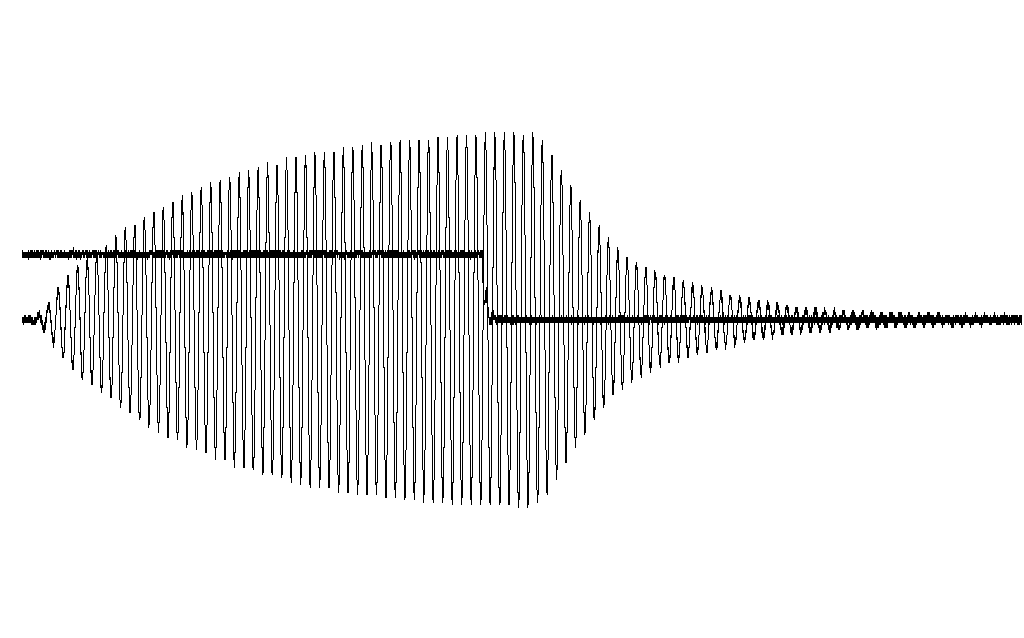
\includegraphics[width=0.8\textwidth]{scope_0.png}
    \captionof{figure}{Signal von der Pickup Probe}
		\label{fig:PP}
	\end{Figure}
Leider ist dies unser einziges gesichertes Bild von dem Singal. Eines mit korrekter Achsenbeschriftung und Skalen wurde nicht gesichert. Es ist allerdings auch hier schon gut zu erkennen, dass das größere Signal, also die Antwort der Pickup Probe, dann abfällt, sobald kein Magnetfeld (das kleine gerade Singal) anliegt.

  Um letztlich die longitunale und transversale Relaxationszeit zu ermitteln müssen wir in der Lage sein unser Medium druch die Spins mit einem Magnetfeld magnetisieren zu können. Dafür haben wir den Magneten und die Helmholzspulen. Mithilfe der Magneten können wir mit dessen homogenen Magnetfeldes eine z-Richtung defnieren und in diese auch unser Medium magnetisieren. Dabei richten sich die Spins, welche ein magnetisches Moment aufgrund des Drehimpulses der Ladung haben, in z-Richtung aus. Nun lässt sich ein zirkular polarisiertes Magenetfeld mithilfe der Helmholzspulen anlegen. Treffen wir mit der Frequenz des zirkluaren Magnetfeldes nun die sog. Lamor-Frequenz, so lässt sich ein Drehmoment auf die Spins ausüben, welches die Ausrichtung der Spins in die xy-Ebene neigt. Die Lamor-Frequen $\omega_0$ ist die gleiche, welche bei einem Übergang von $m_s=+\frac{1}{2}$ zu $m_s=-\frac{1}{2}$ benötigt wird:
\begin{align}
  \Delta U = \hbar \omega_0.
\end{align}
Um nun das Magnetfeld $B_0$ auf die Lamorfrquenz einstellen zu können, müssen wir die Energie berechnen, die uns dann den Übergang geben soll. Dafür nutzen wir die Relationen aus, dass $\bm{\mu}=\gamma \bm{J}$ und $\bm{J}=\hbar\bm{I}$ ist.
\begin{align}
  U &= - \bm{\mu} \cdot \bm{B}\\
    &= - \mu_zB_0\\
    &= - \gamma\hbar I_z B_0
\end{align}
Mit $m_s=\pm \frac{1}{2}$ erhalten wir als Differenz 
\begin{align}
  \Delta U = \gamma \hbar B_0.
\end{align}
Daraus ergibt sich die Bedingung
\begin{align}
  \omega_0 = \gamma B_0.
\end{align}
Je länger wir nun dieses Feld angeschalten lassen, desto größer wird der Neigungswinkel. Dieser Zeitraum wird RF-Pulse genannt und lässt sich an dem Pulse Programmer mit \texttt{A_len} einstellen. Sollten wir einen Neigungswinkel von $\frac{\pi}{2}$ erreichen, so können wir aufgrund der Sample Coil, die über den Reciever verstärkt wird eine Auslänkung auf unserem Oszilloskop sehen. Erreichen wir $\pi$, so wird der Ausschlag wieder 0 sein, da die Sample Coil nur ein Magnetfeld in der xy-Ebene messen kann und nun unsere Magnetisierung in $(-)$z-Richtung ausgerichtet ist. Da allerdings immernoch das homogene Magnetfeld wirkt, richtet sich der Spin nach der Neigung wieder in z-Richtung aus. Dieses Verhalten ist aufgraund der Gesammtmagnetisierung mit der Sample Coil messbar und wird Free Induction Decay (FID) genannt. Wir ersetzen hier die Pickup Probe mit unserer Mineralöl Probe. Nun müssen die Gradienten am PS2 Controller und die Frequenz am Syntheziser so optimiert werden, dass wir ein möglichst langes FID und für den Fall, dass wir bei $\pi$ liegen, eine möglichst kleine Amplitude haben. Gleichzeitig wird das I (In Phase) und Q (Out of Phase) Signal betrachetet, welches keine Nachschwingung haben darf, da dann die Resonazfrequenz getroffen wird. Wir erhalten das in Abb. \ref{fig:opt_sig} dargestellte Signal. Dabei ist eine Frequenz von \SI{21.18322+-0.00001}{\mega Hz} eingestellt. Das I und Q Signal würden dann entsprechend wie bei einem gedämpften harmonischen Oszillator im Kriechfall aussehen.
  \begin{Figure}
    \centering\resizebox{\textwidth}{!}{% GNUPLOT: LaTeX picture with Postscript
\begingroup
  \makeatletter
  \providecommand\color[2][]{%
    \GenericError{(gnuplot) \space\space\space\@spaces}{%
      Package color not loaded in conjunction with
      terminal option `colourtext'%
    }{See the gnuplot documentation for explanation.%
    }{Either use 'blacktext' in gnuplot or load the package
      color.sty in LaTeX.}%
    \renewcommand\color[2][]{}%
  }%
  \providecommand\includegraphics[2][]{%
    \GenericError{(gnuplot) \space\space\space\@spaces}{%
      Package graphicx or graphics not loaded%
    }{See the gnuplot documentation for explanation.%
    }{The gnuplot epslatex terminal needs graphicx.sty or graphics.sty.}%
    \renewcommand\includegraphics[2][]{}%
  }%
  \providecommand\rotatebox[2]{#2}%
  \@ifundefined{ifGPcolor}{%
    \newif\ifGPcolor
    \GPcolortrue
  }{}%
  \@ifundefined{ifGPblacktext}{%
    \newif\ifGPblacktext
    \GPblacktexttrue
  }{}%
  % define a \g@addto@macro without @ in the name:
  \let\gplgaddtomacro\g@addto@macro
  % define empty templates for all commands taking text:
  \gdef\gplbacktext{}%
  \gdef\gplfronttext{}%
  \makeatother
  \ifGPblacktext
    % no textcolor at all
    \def\colorrgb#1{}%
    \def\colorgray#1{}%
  \else
    % gray or color?
    \ifGPcolor
      \def\colorrgb#1{\color[rgb]{#1}}%
      \def\colorgray#1{\color[gray]{#1}}%
      \expandafter\def\csname LTw\endcsname{\color{white}}%
      \expandafter\def\csname LTb\endcsname{\color{black}}%
      \expandafter\def\csname LTa\endcsname{\color{black}}%
      \expandafter\def\csname LT0\endcsname{\color[rgb]{1,0,0}}%
      \expandafter\def\csname LT1\endcsname{\color[rgb]{0,1,0}}%
      \expandafter\def\csname LT2\endcsname{\color[rgb]{0,0,1}}%
      \expandafter\def\csname LT3\endcsname{\color[rgb]{1,0,1}}%
      \expandafter\def\csname LT4\endcsname{\color[rgb]{0,1,1}}%
      \expandafter\def\csname LT5\endcsname{\color[rgb]{1,1,0}}%
      \expandafter\def\csname LT6\endcsname{\color[rgb]{0,0,0}}%
      \expandafter\def\csname LT7\endcsname{\color[rgb]{1,0.3,0}}%
      \expandafter\def\csname LT8\endcsname{\color[rgb]{0.5,0.5,0.5}}%
    \else
      % gray
      \def\colorrgb#1{\color{black}}%
      \def\colorgray#1{\color[gray]{#1}}%
      \expandafter\def\csname LTw\endcsname{\color{white}}%
      \expandafter\def\csname LTb\endcsname{\color{black}}%
      \expandafter\def\csname LTa\endcsname{\color{black}}%
      \expandafter\def\csname LT0\endcsname{\color{black}}%
      \expandafter\def\csname LT1\endcsname{\color{black}}%
      \expandafter\def\csname LT2\endcsname{\color{black}}%
      \expandafter\def\csname LT3\endcsname{\color{black}}%
      \expandafter\def\csname LT4\endcsname{\color{black}}%
      \expandafter\def\csname LT5\endcsname{\color{black}}%
      \expandafter\def\csname LT6\endcsname{\color{black}}%
      \expandafter\def\csname LT7\endcsname{\color{black}}%
      \expandafter\def\csname LT8\endcsname{\color{black}}%
    \fi
  \fi
    \setlength{\unitlength}{0.0500bp}%
    \ifx\gptboxheight\undefined%
      \newlength{\gptboxheight}%
      \newlength{\gptboxwidth}%
      \newsavebox{\gptboxtext}%
    \fi%
    \setlength{\fboxrule}{0.5pt}%
    \setlength{\fboxsep}{1pt}%
    \definecolor{tbcol}{rgb}{1,1,1}%
\begin{picture}(7200.00,4320.00)%
    \gplgaddtomacro\gplbacktext{%
      \csname LTb\endcsname%%
      \put(731,619){\makebox(0,0)[r]{\strut{}$-0.2$}}%
      \csname LTb\endcsname%%
      \put(731,1006){\makebox(0,0)[r]{\strut{}$0$}}%
      \csname LTb\endcsname%%
      \put(731,1394){\makebox(0,0)[r]{\strut{}$0.2$}}%
      \csname LTb\endcsname%%
      \put(731,1781){\makebox(0,0)[r]{\strut{}$0.4$}}%
      \csname LTb\endcsname%%
      \put(731,2169){\makebox(0,0)[r]{\strut{}$0.6$}}%
      \csname LTb\endcsname%%
      \put(731,2556){\makebox(0,0)[r]{\strut{}$0.8$}}%
      \csname LTb\endcsname%%
      \put(731,2944){\makebox(0,0)[r]{\strut{}$1$}}%
      \csname LTb\endcsname%%
      \put(731,3331){\makebox(0,0)[r]{\strut{}$1.2$}}%
      \csname LTb\endcsname%%
      \put(731,3718){\makebox(0,0)[r]{\strut{}$1.4$}}%
      \csname LTb\endcsname%%
      \put(731,4106){\makebox(0,0)[r]{\strut{}$1.6$}}%
      \csname LTb\endcsname%%
      \put(829,425){\makebox(0,0){\strut{}$-20$}}%
      \csname LTb\endcsname%%
      \put(1380,425){\makebox(0,0){\strut{}$-15$}}%
      \csname LTb\endcsname%%
      \put(1931,425){\makebox(0,0){\strut{}$-10$}}%
      \csname LTb\endcsname%%
      \put(2481,425){\makebox(0,0){\strut{}$-5$}}%
      \csname LTb\endcsname%%
      \put(3032,425){\makebox(0,0){\strut{}$0$}}%
      \csname LTb\endcsname%%
      \put(3582,425){\makebox(0,0){\strut{}$5$}}%
      \csname LTb\endcsname%%
      \put(4133,425){\makebox(0,0){\strut{}$10$}}%
      \csname LTb\endcsname%%
      \put(4683,425){\makebox(0,0){\strut{}$15$}}%
      \csname LTb\endcsname%%
      \put(5234,425){\makebox(0,0){\strut{}$20$}}%
      \csname LTb\endcsname%%
      \put(5785,425){\makebox(0,0){\strut{}$25$}}%
      \csname LTb\endcsname%%
      \put(6335,425){\makebox(0,0){\strut{}$30$}}%
      \csname LTb\endcsname%%
      \put(6886,425){\makebox(0,0){\strut{}$35$}}%
    }%
    \gplgaddtomacro\gplfronttext{%
      \csname LTb\endcsname%%
      \put(6123,3932){\makebox(0,0)[r]{\strut{}FID}}%
      \csname LTb\endcsname%%
      \put(170,2362){\rotatebox{-270.00}{\makebox(0,0){\strut{}Auslenkung/\SI{}{V}}}}%
      \csname LTb\endcsname%%
      \put(3858,135){\makebox(0,0){\strut{}Zeit t/\SI{}{\micro s}}}%
    }%
    \gplbacktext
    \put(0,0){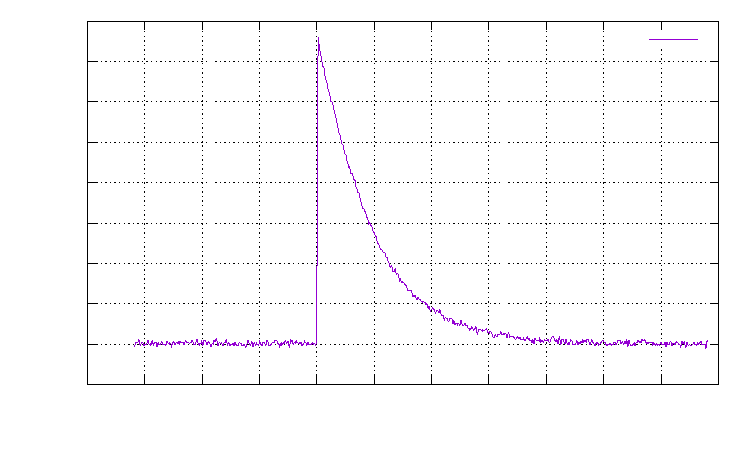
\includegraphics[width={360.00bp},height={216.00bp}]{opt_sig}}%
    \gplfronttext
  \end{picture}%
\endgroup
}
    \captionof{figure}{
      Optimiertes FID Signal.
    }
    \label{fig:opt_sig}
  \end{Figure}
  Generell messen wir aufgrund des Farady'schen Gesetzes $U=-\frac{\text{d}}{\text{d}t}\Phi_m$ eine Spannung. Das liegt daran, dass der Spin wegen des Drehimpulses um die z-Achse präzediert und so $\Phi_m$ sich zeitlich ändert. Dabei hatten wir sichergestellt, dass die Zerfallszeit über \SI{4}{\milli s} liegt.

  Nun mussten die Pulslängen ermittelt werden, dafür wurde diese so eingestellt, dass wir die Amplitude minimieren. Somit erhalten wir ein $\pi$-Puls. Währendessen verändern sich die Nachschwingungen von I und Q. Nun hablieren wir diese Pulslänge und erhalten ein $\frac{\pi}{2}$-Puls. Die Pulslängen sind dabei \SI{2.42}{\milli s} bzw. \SI{4.84}{\milli s}. Hierbei und bei allen folgenden Messungen wurde das Offset direkt im Versuch abgezogen und ist somit in der eigenen Unsicherheitenabschätzung schon mit einbezogen. Dabei erhalten wir ein Amplitudenverhältniss $U_{\text{max}}(\pi):U_{\text{max}}(\pi/2)$ von 1:\SI{17.2+-1.4} mit $U_{\text{max}}(\pi)=\SI{0.086+-0.007}{V}$ und $U_{\text{max}}(\pi/2)=\SI{1.483+-0.007}{V}$, was über den notwendigen 1:6 liegt.


  \subsection{Rabi-Oszillationen}
  Bei der Rabi-Oszillation erhöhen wir die Pulslänge und messen die Maxima, also die Amplitude. Wir stellen sicher, dass die Periode zwischen zwei Pulsen mit \SI{1}{s} ausreichend groß ist. Neben der FID Amplitude wir auch die Amplitude des In-Signals gemessen. Wir wählen hierbei Pulslängen von zwischen \SI{0.5}{\micro s} und \SI{12}{\micro s}. Dabei erhalten wir Abb. \ref{fig:rabioszi}.
  \begin{Figure}
    \centering\resizebox{\textwidth}{!}{% GNUPLOT: LaTeX picture with Postscript
\begingroup
  \makeatletter
  \providecommand\color[2][]{%
    \GenericError{(gnuplot) \space\space\space\@spaces}{%
      Package color not loaded in conjunction with
      terminal option `colourtext'%
    }{See the gnuplot documentation for explanation.%
    }{Either use 'blacktext' in gnuplot or load the package
      color.sty in LaTeX.}%
    \renewcommand\color[2][]{}%
  }%
  \providecommand\includegraphics[2][]{%
    \GenericError{(gnuplot) \space\space\space\@spaces}{%
      Package graphicx or graphics not loaded%
    }{See the gnuplot documentation for explanation.%
    }{The gnuplot epslatex terminal needs graphicx.sty or graphics.sty.}%
    \renewcommand\includegraphics[2][]{}%
  }%
  \providecommand\rotatebox[2]{#2}%
  \@ifundefined{ifGPcolor}{%
    \newif\ifGPcolor
    \GPcolortrue
  }{}%
  \@ifundefined{ifGPblacktext}{%
    \newif\ifGPblacktext
    \GPblacktexttrue
  }{}%
  % define a \g@addto@macro without @ in the name:
  \let\gplgaddtomacro\g@addto@macro
  % define empty templates for all commands taking text:
  \gdef\gplbacktext{}%
  \gdef\gplfronttext{}%
  \makeatother
  \ifGPblacktext
    % no textcolor at all
    \def\colorrgb#1{}%
    \def\colorgray#1{}%
  \else
    % gray or color?
    \ifGPcolor
      \def\colorrgb#1{\color[rgb]{#1}}%
      \def\colorgray#1{\color[gray]{#1}}%
      \expandafter\def\csname LTw\endcsname{\color{white}}%
      \expandafter\def\csname LTb\endcsname{\color{black}}%
      \expandafter\def\csname LTa\endcsname{\color{black}}%
      \expandafter\def\csname LT0\endcsname{\color[rgb]{1,0,0}}%
      \expandafter\def\csname LT1\endcsname{\color[rgb]{0,1,0}}%
      \expandafter\def\csname LT2\endcsname{\color[rgb]{0,0,1}}%
      \expandafter\def\csname LT3\endcsname{\color[rgb]{1,0,1}}%
      \expandafter\def\csname LT4\endcsname{\color[rgb]{0,1,1}}%
      \expandafter\def\csname LT5\endcsname{\color[rgb]{1,1,0}}%
      \expandafter\def\csname LT6\endcsname{\color[rgb]{0,0,0}}%
      \expandafter\def\csname LT7\endcsname{\color[rgb]{1,0.3,0}}%
      \expandafter\def\csname LT8\endcsname{\color[rgb]{0.5,0.5,0.5}}%
    \else
      % gray
      \def\colorrgb#1{\color{black}}%
      \def\colorgray#1{\color[gray]{#1}}%
      \expandafter\def\csname LTw\endcsname{\color{white}}%
      \expandafter\def\csname LTb\endcsname{\color{black}}%
      \expandafter\def\csname LTa\endcsname{\color{black}}%
      \expandafter\def\csname LT0\endcsname{\color{black}}%
      \expandafter\def\csname LT1\endcsname{\color{black}}%
      \expandafter\def\csname LT2\endcsname{\color{black}}%
      \expandafter\def\csname LT3\endcsname{\color{black}}%
      \expandafter\def\csname LT4\endcsname{\color{black}}%
      \expandafter\def\csname LT5\endcsname{\color{black}}%
      \expandafter\def\csname LT6\endcsname{\color{black}}%
      \expandafter\def\csname LT7\endcsname{\color{black}}%
      \expandafter\def\csname LT8\endcsname{\color{black}}%
    \fi
  \fi
    \setlength{\unitlength}{0.0500bp}%
    \ifx\gptboxheight\undefined%
      \newlength{\gptboxheight}%
      \newlength{\gptboxwidth}%
      \newsavebox{\gptboxtext}%
    \fi%
    \setlength{\fboxrule}{0.5pt}%
    \setlength{\fboxsep}{1pt}%
    \definecolor{tbcol}{rgb}{1,1,1}%
\begin{picture}(7200.00,4320.00)%
    \gplgaddtomacro\gplbacktext{%
      \csname LTb\endcsname%%
      \put(731,619){\makebox(0,0)[r]{\strut{}$-400$}}%
      \csname LTb\endcsname%%
      \put(731,967){\makebox(0,0)[r]{\strut{}$-200$}}%
      \csname LTb\endcsname%%
      \put(731,1316){\makebox(0,0)[r]{\strut{}$0$}}%
      \csname LTb\endcsname%%
      \put(731,1665){\makebox(0,0)[r]{\strut{}$200$}}%
      \csname LTb\endcsname%%
      \put(731,2014){\makebox(0,0)[r]{\strut{}$400$}}%
      \csname LTb\endcsname%%
      \put(731,2362){\makebox(0,0)[r]{\strut{}$600$}}%
      \csname LTb\endcsname%%
      \put(731,2711){\makebox(0,0)[r]{\strut{}$800$}}%
      \csname LTb\endcsname%%
      \put(731,3060){\makebox(0,0)[r]{\strut{}$1000$}}%
      \csname LTb\endcsname%%
      \put(731,3409){\makebox(0,0)[r]{\strut{}$1200$}}%
      \csname LTb\endcsname%%
      \put(731,3757){\makebox(0,0)[r]{\strut{}$1400$}}%
      \csname LTb\endcsname%%
      \put(731,4106){\makebox(0,0)[r]{\strut{}$1600$}}%
      \csname LTb\endcsname%%
      \put(829,425){\makebox(0,0){\strut{}$0$}}%
      \csname LTb\endcsname%%
      \put(1839,425){\makebox(0,0){\strut{}$2$}}%
      \csname LTb\endcsname%%
      \put(2848,425){\makebox(0,0){\strut{}$4$}}%
      \csname LTb\endcsname%%
      \put(3858,425){\makebox(0,0){\strut{}$6$}}%
      \csname LTb\endcsname%%
      \put(4867,425){\makebox(0,0){\strut{}$8$}}%
      \csname LTb\endcsname%%
      \put(5876,425){\makebox(0,0){\strut{}$10$}}%
      \csname LTb\endcsname%%
      \put(6886,425){\makebox(0,0){\strut{}$12$}}%
    }%
    \gplgaddtomacro\gplfronttext{%
      \csname LTb\endcsname%%
      \put(6123,3932){\makebox(0,0)[r]{\strut{}Probe}}%
      \csname LTb\endcsname%%
      \put(6123,3738){\makebox(0,0)[r]{\strut{}Probe fit}}%
      \csname LTb\endcsname%%
      \put(6123,3545){\makebox(0,0)[r]{\strut{}In-Phase}}%
      \csname LTb\endcsname%%
      \put(6123,3351){\makebox(0,0)[r]{\strut{}In-Phase fit}}%
      \csname LTb\endcsname%%
      \put(170,2362){\rotatebox{-270.00}{\makebox(0,0){\strut{}Amplitude/$\SI{}{\milli V}$}}}%
      \csname LTb\endcsname%%
      \put(3858,135){\makebox(0,0){\strut{}Pulslänge \texttt{A_len}/$\SI{}{\micro s}$}}%
    }%
    \gplbacktext
    \put(0,0){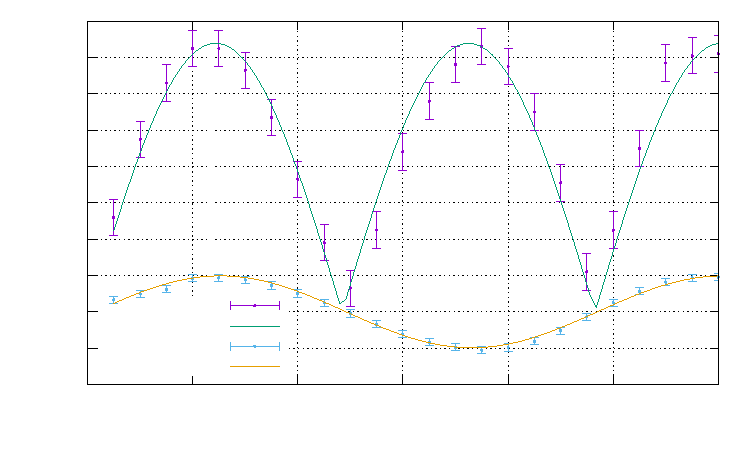
\includegraphics[width={360.00bp},height={216.00bp}]{rabi_oszi}}%
    \gplfronttext
  \end{picture}%
\endgroup
}
    \captionof{figure}{
      Rabi-Oszillation 
    }
    \label{fig:rabioszi}
  \end{Figure}
  Als Anpassfunktionen haben wir für die Probe $f(x)=m\cdot|\sin{(b\cdot x+c)}|$ und für das In-Phase Signal $g(x)=m\cdot\sin{(b\cdot x+c)}$ gewählt. Die Paramter der Anpassung sind in Tab. \ref{Tab:rabioszi} dargestellt.
  \begin{center}
    \begin{tabular}{c|cc}
    & Probe & In-Phase \\
    \hline
    red. $\chi^2$ & 1.03 & 0.46 \\
    $m$ & \SI{1478 \pm 29}{\milli\volt} & \SI{197.9 \pm 3.9}{\milli\volt} \\
    $b$ & \SI{0.6530 \pm 0.0060}{\per\micro\second} & \SI{0.6571 \pm 0.0059}{\per\micro\second} \\
    $c$ & \SI{-0.021 \pm 0.042}{} & \SI{-0.090 \pm 0.041}{}
\end{tabular}
  \captionof{table}{Parameter der Anpassung zu Rabi Oszillation}
  \label{Tab:rabioszi}
  \end{center}
  Ein gutes reduziertes $\chi^2$ liegt in der Nähe von 1. Dies ist für die Probe der Fall mit $1.03$. Für das In-Phase Signal erhalten wir $\chi^2/\text{ddof}=0.46$, was unter unseren gewollten 1 liegt, aber immernoch vertretbar ist. Somit haben wir entweder bei dem In-Phase Signal unsere Messunsicherheit unterschätzt, oder gute Messergebnisse erhalten.

  Wie erwartet, erhalten wir einen Sinus -- mit und ohne Betrag -- welcher Phasengleich ist und die gleiche Periodendauer hat. Dies liegt daran, dass das Antwortsignal den Betrag der Projektion der Magnetisierung in die xy-Ebene und das I Signal die Magnetisierung in y-Richtung zeigt.


  


\end{multicols}
\printbibliography

\end{document}
